\documentclass[11pt]{article}
\usepackage[top=1in,bottom=1in,left=1in,right=1in]{geometry}
\usepackage{Sweave,natbib,amsmath,url}
\usepackage{hyperref} 
\hypersetup{colorlinks,% 
citecolor=black,% 
filecolor=black,% 
linkcolor=black,% 
urlcolor=black } 
\setcounter{tocdepth}{1}

\title{Individual Patient Data Meta-Analysis of Time-to-Events}
\author{Stephanie A. Kovalchik, \url{skoval@ucla.edu}}
\date{\today}

\begin{document}

\maketitle

The package \texttt{ipdmeta} provides methods for conducting a complete
patient-level analysis and a  mixed-level
meta-analysis when the primary endpoint is a time-to-event. The
setting assumed is where the studies to be combined are randomized
controlled intervention trials. For the mixed-level meta-analysis,
aggregate-data trials are multivariate survival estimates (points
along a KM plot) within-intervention, within-trial. In this vignette, extended examples with explanations are
provided for the analytical functions \texttt{coxmcem} and
\texttt{mlma}, for a full IPD and mixed-level meta-analysis, respectively.

\documentclass[11pt]{article}
\usepackage[top=1in,bottom=1in,left=1in,right=1in]{geometry}
\usepackage{Sweave,natbib,amsmath,url}
\usepackage{hyperref} 
\hypersetup{colorlinks,% 
citecolor=black,% 
filecolor=black,% 
linkcolor=black,% 
urlcolor=black } 
\setcounter{tocdepth}{1}

\title{Individual Patient Data Meta-Analysis of Time-to-Events}
\author{Stephanie A. Kovalchik, \url{skoval@ucla.edu}}
\date{\today}

\begin{document}

\maketitle

The package \texttt{ipdmeta} provides methods for conducting a complete
patient-level analysis and a  mixed-level
meta-analysis when the primary endpoint is a time-to-event. The
setting assumed is where the studies to be combined are randomized
controlled intervention trials. For the mixed-level meta-analysis,
aggregate-data trials are multivariate survival estimates (points
along a KM plot) within-intervention, within-trial. In this vignette, extended examples with explanations are
provided for the analytical functions \texttt{coxmcem} and
\texttt{mlma}, for a full IPD and mixed-level meta-analysis, respectively.

\documentclass[11pt]{article}
\usepackage[top=1in,bottom=1in,left=1in,right=1in]{geometry}
\usepackage{Sweave,natbib,amsmath,url}
\usepackage{hyperref} 
\hypersetup{colorlinks,% 
citecolor=black,% 
filecolor=black,% 
linkcolor=black,% 
urlcolor=black } 
\setcounter{tocdepth}{1}

\title{Individual Patient Data Meta-Analysis of Time-to-Events}
\author{Stephanie A. Kovalchik, \url{skoval@ucla.edu}}
\date{\today}

\begin{document}

\maketitle

The package \texttt{ipdmeta} provides methods for conducting a complete
patient-level analysis and a  mixed-level
meta-analysis when the primary endpoint is a time-to-event. The
setting assumed is where the studies to be combined are randomized
controlled intervention trials. For the mixed-level meta-analysis,
aggregate-data trials are multivariate survival estimates (points
along a KM plot) within-intervention, within-trial. In this vignette, extended examples with explanations are
provided for the analytical functions \texttt{coxmcem} and
\texttt{mlma}, for a full IPD and mixed-level meta-analysis, respectively.

\documentclass[11pt]{article}
\usepackage[top=1in,bottom=1in,left=1in,right=1in]{geometry}
\usepackage{Sweave,natbib,amsmath,url}
\usepackage{hyperref} 
\hypersetup{colorlinks,% 
citecolor=black,% 
filecolor=black,% 
linkcolor=black,% 
urlcolor=black } 
\setcounter{tocdepth}{1}

\title{Individual Patient Data Meta-Analysis of Time-to-Events}
\author{Stephanie A. Kovalchik, \url{skoval@ucla.edu}}
\date{\today}

\begin{document}

\maketitle

The package \texttt{ipdmeta} provides methods for conducting a complete
patient-level analysis and a  mixed-level
meta-analysis when the primary endpoint is a time-to-event. The
setting assumed is where the studies to be combined are randomized
controlled intervention trials. For the mixed-level meta-analysis,
aggregate-data trials are multivariate survival estimates (points
along a KM plot) within-intervention, within-trial. In this vignette, extended examples with explanations are
provided for the analytical functions \texttt{coxmcem} and
\texttt{mlma}, for a full IPD and mixed-level meta-analysis, respectively.

\input{ipdmeta_vignette.toc}

\clearpage

\section{Estimation for Cox Mixed Effects Model: coxmcem}

\input{coxmcem}

\section{Mixed-level Meta-analysis: mlma}

\input{mlma}

\clearpage

\begin{figure}\center
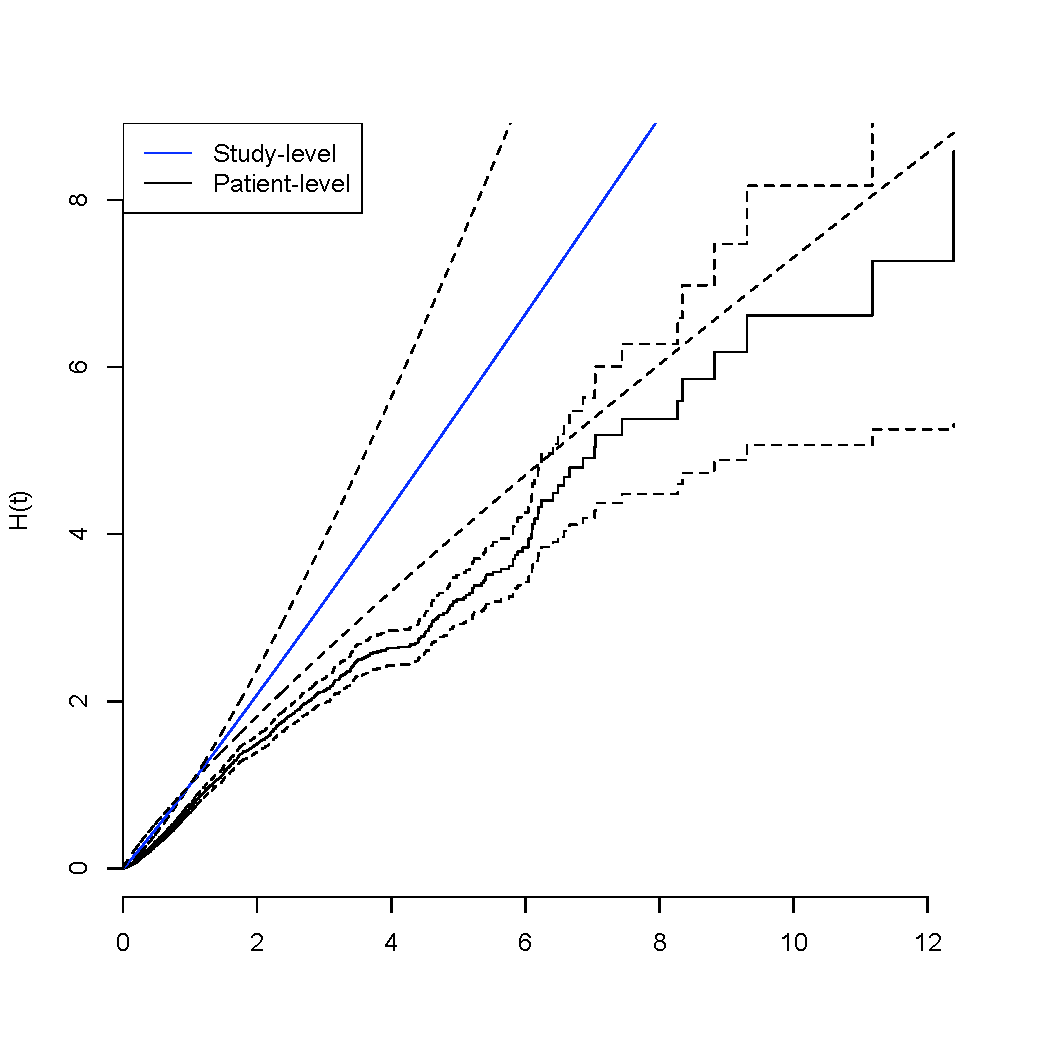
\includegraphics{haz.pdf}
\caption{Baseline hazard estimated by study-level and patient-level
  models of mixed-level meta-analysis. Dotted lines denote the 95\% CI.}
\end{figure}

\clearpage

\label{ref:ref}

\bibliographystyle{wileyj}

\bibliography{/Users/skoval/meta/bib/survival,/Users/skoval/meta/bib/survival.meta,/Users/skoval/meta/bib/statistics,/Users/skoval/meta/bib/meta,/Users/skoval/meta/bib/ecological_bias,/Users/skoval/meta/bib/likelihood,/Users/skoval/meta/bib/bayes.meta,/Users/skoval/meta/bib/bayes,/Users/skoval/meta/bib/power_loss,/Users/skoval/meta/bib/cox_randomeffects,/Users/skoval/meta/bib/importance_sampling,/Users/skoval/bibliography/public_health,/Users/skoval/bibliography/cer,/Users/skoval/meta/bib/bhits}


\end{document}


\clearpage

\section{Estimation for Cox Mixed Effects Model: coxmcem}

\subsection{Description}

The Cox mixed effects model is an extension of the standard Cox
regression model for censored data \cite{Cox1972a,Cox1975a}. It
suitable for censored data where the unit of analysis is clustered in
some way, for example, children within households. It builds on
frailty models by allowing for more complex random effects structures
corresponding to more complex grouping, for example, twins among
siblings within household. The general framework has also been
described as a proportional hazards mixed model or multivariate
frailty model. 

Estimation approaches have included approximate and sampling
methods. Approximate methods are based on a Laplace approximation to
the marginal log-likelihood \cite{Ripatti2000a}. This is implemented
by the package \texttt{coxme} of Therneau \cite{Therneau2009a}. It is well-known that the
loss of information with the approximation results in an
underestimation of the parameter standard errors \cite{Abrahantes2007a}.

Sampling methods take an expectation-maximization approach which has
the advantage of retaining all information on the model
parameters. Sampling is required at the E-step. Vaida and Xu (2000) propose
a Gibbs adaptive rejection sampling method to sample the posterior
frailties given a multivariate-normal prior \cite{Vaida2000a}. This
approach is implemented with the package \texttt{phmm}
\cite{Donohue2010a}. Ripatti, Larsen and Palmgren (2002) suggest a rejection sampler; the author is not
aware of any software for this strategy \cite{Ripatti2002a}. The difficulty
with sampling approaches is that convergence has to be checked at the
E-step and is a challenge to automate. 

The \texttt{coxmcem} uses importance sampling to obtain averages for
the multivariate frailties at the E-step. Booth and Hobert (1999) give a description of
the general approach for generalized linear mixed models
\cite{Booth1999a}. The appeal of an importance-sample is that it obviates the need for
convergence to the target distribution while retaining all information
about the model parameters. The proposal density for the
\texttt{coxmcem} implementation is a
multivariate T whose location is the maximum-likelihood estimate of
the frailties at the current EM iteration. Monitoring the MC error and
parameter estimates follows the procedure outlined by Ripatti~\emph{et
  al.} (2002). 


\subsection{Usage}

I illustrate the use of \texttt{coxmcem}. An often used test case for
frailty models is a data set of time to tumor occurrence for 50 litters of
rats \cite[chapter 9]{Therneau2000a}, with one of three rats in each litter randomly selected to recieve
a
carcinogen exposure \citep{Mantel1977a}. This is the data that will be
used for the case study. The first few rows are given below

\begin{Schunk}
\begin{Sinput}
library(ipdmeta)
data(cancer.rats)
head(cancer.rats)
  litter rx time event
1      1  1  101      0
2      1  0   49      1
3      1  0  104      0
4      2  1  104      0
5      2  0  102      0
6      2  0  104      0
\end{Sinput}
\end{Schunk}

\subsubsection{Model}

The PHMM model for time-to-tumor occurence for the
\texttt{cancer.rats} data is

\begin{equation}
\label{eq:uni}
\lambda(t) = \lambda_0(t) \mbox{exp}\lbrace x_{rx,i} \beta + b_{k(i)} \rbrace
\end{equation}

\noindent where $x_{rx,i}$ is the ith rat's indicator for carcinogen
exposure and $b_k$ is the kth litter frailty with ith subject litter
membership k(i). All K = 50 frailties share the normal distribution $b_k \sim N(0,\sigma^2)$. 

\subsubsection{Implementation}

PHMM (\ref{eq:uni}) with importance sampling is implemented as follows

\begin{Schunk}
\begin{Sinput}
set.seed(123321)

fit <- coxmcem(
    Surv(time,event)~rx,
    random=~(1|litter),
    n.groups=50,
    data=cancer.rats,
    max.iter=20,
    min.sample=500,
    mc.step=2,
    est.delta=1/100,
    df=30
)
\end{Sinput}
\end{Schunk}

The formula for the survival object is the same as would be supplied
to any of the models of \texttt{survival}. The random formula
indicated the frailty structure. Here I specifiy a baseline frailty
by litter. The number of groups is the number of clusters in the data
set. In this case clustering is by litter and there are 50 total
litters. Next, I indicate the name of the data frame containing the
variables described in the model formulas.

The remaining arguments determine the stopping rule for the EM
importance sampling procedure. The argument \texttt{min.sample}
indicates the number of draws from the joint T distribution for the
frailties that are generated at each E step. The sample determines the
number of frailties in the Monte Carlo estimate of the averages for
the complete log-likelihood. It is typical to begin with a small
number while the model estimates are far from the MLE and increase the
sample with the algorithm iterations. In this case I specify a
starting sample size of 1000. Because the algorithm will run more
slowly with a larger sample size, it is best to begin with a small
number, say 200, if suitable choices for some of the arguments,
i.e. \texttt{df}, are still being worked out.

Convergence of the algorithm is judged by the relative change of the
model paramters. Denote the set of fixed effects and frailty variance
parameters as $\theta$. In this example $\theta$ consists of the fixed
effects estimate for the treatment effect \texttt{rx} and univariate
frailty variance $\texttt{vcov} = \sigma^2$. The relative change in each parameter from the
previous iteration is determined. If the maximum change among all
parameters is less than \texttt{est.delta}, \emph{for three
  consecutive iterations}, then the algorithm
stops. With a setting for \texttt{est.delta} of $\frac{1}{100}$ this
would mean that a less than 1\% relative change for all parameters is
required for three iterations in a row in order to stop. For this
reason, the minimum number of iterations for any implementation is three.

If \texttt{max.iter} is reached before the convergence threshold has
been met, the algorithm stops.

The argument \texttt{mc.step} determines how the E-step frailty sample
size is increased. When the coefficient of variation of the relative
change of the parameters is large, this suggests that the MC error is
too large and the sample size should be increased. Thus, when the
three most recent relative change between consecutive EM estimates
have a coefficient of variation greater than unity, the current sample
size of N is increased by 

\[
N = N + \frac{1}{\mbox{mc.step}}N
\]


\subsubsection{Summary}

First I review the algorithm properties to see if enough iterations
and MC samples have been obtained. 

\begin{Schunk}
\begin{Sinput}
fit[1:5]
$max.weight
[1] 0.01193944 0.01176729 0.01087182

$mc.samples
[1] 500 500 500

$est.converge
[1] 0.006424424 0.009711094 0.001660967

$loglik
[1] -177.5236 -177.7699 -177.8148

$sd.loglik
[1] 9.276321 8.759723 8.369623
\end{Sinput}
\end{Schunk}

The algorithm stopped after 3 iterations, the minimum possible, so
that the MC sample size never exceeded the initial starting value. The
maximum weights are the maximum weights among all importance weights
for the given iteration. These will each be a value between (0,1)
since the sum of all importance weights are 1, their being
normalized. For a sample size of N, each iteration draws N joint
frailties, in this case 500 vectors of 50 frailties. Averages of the frailties are
the importance-weighted average of the N-size sample. No single set of
frailties should dominate this average so it needs to be checked that
the weights are fairly evenly distributed. If the weights were all
equal, each would be $\frac{1}{N}$. A maximum weight much greater than
this would suggest that some adjustments were needed in the model of T
proposal distribution settings. Here I see that no single draw
contributed greater than approximately 1\% to the average so the
algorithm settings seem to be fine.

The standard deviation of the log-likelihood can complement the
interpretation of the importance weights. These are the standard
deviations of the conditional log-likelihood of the PHMM conditional
on each
sample frailty of the given iteration. There should be enough
variation in the frailties to be sure that the full support is
represented. However, large variation could produce great imbalances
in the importance weights. So if the \texttt{max.weights} seem large, and the
standard deviation of the log-likelihoods are large relative to the
MLE log-likelihood values, this would suggest that the T proposal
settings need to be modified or that the model has been poorly
specified. For example, one way to reduce variation in the frailty
proposal would be to lower the \texttt{df}. In general, a good
starting place might be to set \texttt{df} to the number of clusters
in the data set, approximately.

Regarding the model estimates, I find that the final iteration
stopped with a relative maximal change of 0.17\%, meaning that both
the \texttt{coef} and \texttt{vcov} estimates had less than 0.2\% change
from the previous iteration values. By specifying a \texttt{est.delta}
of 1\%, I required that the algorithm proceed until three consecutive
relative changes had maximum differences of 1\% or less. This was met
after the minimum three iterations in this case.

Being satisfied with the convergence properties of the MCEM I now
consider the findings. The fixed effect estimates are the list element \texttt{coef} and the
frailty variance parameters \texttt{vcov}.

\begin{Schunk}
\begin{Sinput}
> fit$coef
      rx 
0.910061 

> fit$vcov
          [,1]
[1,] 0.4316714
\end{Sinput}
\end{Schunk}

Variances for each of these parameters are contained in the list
\texttt{var}. A large-sample 95\% CI for the hazard ratio
of tumor occurrence given carcinogen exposure can be obtained with the
following code. I show the do-it-yourself way then a version which
makes  use of the confidence interval function \texttt{ci}.

\begin{Schunk}
\begin{Sinput}
> exp(fit$coef+c(-2,2)*sqrt(fit$var$coef))
[1] 1.300951 4.744692

> ci(1,fit$coef,fit$var$coef)
      low point.est      high 
 1.317909  2.484474  4.683640 
\end{Sinput}
\end{Schunk}

The interpretation is that there is a 2.5 increased risk to developing
a tumor for rats exposed to the carcinogen which can be stated with
95\% confidence.

The variability between litters in baseline risk was

\begin{Schunk}
\begin{Sinput}
sqrt(fit$vcov)
         [,1]
[1,] 0.657017

> ci(1,0,fit$vcov,alpha=.3)
      low point.est      high 
0.5061337 1.0000000 1.9757625 
\end{Sinput}
\end{Schunk}

\noindent suggesting that there is a roughly 30\% chance that
otherwise equivalent rats with respect to exposure could have a
relative hazard outside of the interval (0.51, 1.98), with 30\%
probability, which seems a substantial level of heterogeneity.

A Wald test for the significance of the fixed effects can be obtained
by computing the Wald test-statistics using the variances of the
\texttt{coef}.

\begin{Schunk}
\begin{Sinput}
> fit$coef/sqrt(get.diag(fit$var$coef))
      rx 
2.813322 

> p.value <- pnorm(abs(fit$coef/sqrt(get.diag(fit$var$coef))),lower=FALSE)
> p.value
         rx 
0.002451630 
\end{Sinput}
\end{Schunk}

Testing of the random effect is more challenging because of the
asymptotic properties of common tests when the variance parameter is
near the boundary, that is, the null hypothesis that the variance is
zero. A Wald test can be a useful exploratory tool but a likelihood
ratio test is generally preferred \cite{Self1987a}.

\begin{Schunk}
\begin{Sinput}
> fit$vcov/sqrt(fit$var$vcov)
         [,1]
[1,] 1.868417
\end{Sinput}
\end{Schunk}

This gives support for the inclusion of the baseline litter random
effect. 

\subsubsection{Recognizing a Poorly Specified Model}

I now consider how to identify a poorly fit model when the random
effect and fixed effects structures have been misspecified. I do this
be introducing an unrelated variable into the model. The `noise' term
is included as a fixed and random effect.

\begin{equation}
\label{eq:uni}
\lambda(t) = \lambda_0(t) \mbox{exp}\lbrace x_{rx,i} \beta_1 +
x_{noise,i} \beta_2 + b_{k(i),1} +  b_{k(i),2} x_{noise,i} \rbrace
\end{equation}

\noindent with 

\[
\begin{pmatrix} b_{k,1} \\ b_{k,2} \end{pmatrix} \sim
MVN(\mathbf{0},\begin{pmatrix} \theta_1 & \theta_3 \\
\theta_3 & \theta_2 \end{pmatrix})
\]

\noindent And the implemenation is given by 

\begin{Schunk}
\begin{Sinput}
set.seed(456654)

cancer.rats$noise <- runif(150)

fit <- coxmcem(
    Surv(time,event)~rx+noise,
    random=~(1+noise|litter),
    n.groups=50,
    data=cancer.rats,
    max.iter=10,
    min.sample=300,
    mc.step=2,
    est.delta=1/100,
    df=30
)
\end{Sinput}
\end{Schunk}

Since I am initially unsure about the fit of this model, I do a
trial run with a smaller initial sample size and fewer
iterations. Monitoring the relative change in estimates I note some
cases of high change. One way in which this could occur is when a
parameter of the model is close to zero, so that small absolute
changes in estimates result in large relative changes.

I also note some iterations with high \texttt{max.weight} and
\texttt{sd.loglik}. Looking at the fixed effect estimates, I conclude
that the \texttt{noise} term is not contributing any information to the
tumor-occurrence outcome and that the large relative changes in the
parameters (large \texttt{est.delta}) was due to the noise coefficient
being near to zero.

\begin{Schunk}
\begin{Sinput}
> fit$coef/sqrt(get.diag(fit$var$coef))
      rx    noise 
3.019627 0.642682 
\end{Sinput}
\end{Schunk}


\section{Mixed-level Meta-analysis: mlma}

Mixed-level meta-analysis (MLMA) describes a quantitative summary of
evidence at disparate levels with some trials providing
individual-level data and other trials summary data. The \texttt{mlma}
function performs MLMA estimation when the outcome is a time-to-event
and aggregate data is in the form of a set of survival estimates
within treatment group, within study. 

The individual patient data (IPD) model is a proportional hazards
mixed model (PHMM) allowing a general random effects structure with multivariate normal
frailties. The study-level model is a multivariate mixed model on the
complementary-log-log of the study-specific survival estimates. This
study-level model is the implied linear relation based on the
assumption that all outcomes follow the PHMM at the patient level. 

Through
combined likelihood maximization, both evidence levels contribute to
the estimation of shared fixed effects and the frailty variance
structures. The estimation uses an MCEM approach with importance
sampling following the same procedure are for the PHMM analysis
implemented by \texttt{coxmcem}. Separation of the patient-level and study-level effects is
also possible if there is concern of non-equivalence in the risk
associations at the aggregate level versus the subject level.

\subsection{Usage}

Consider a mixed-level dataset consisting of 8 IPD and 2
study-level RCTs. The model for the PHMM has treatment main effect. A bivariate frailty
for baseline and treatment effect by trial is the random component.

See \texttt{example(ipd.data)} and \texttt{example(meta.data)} for a
quick visual display of the nature of the mixed-level data for this
example.

To obtain the MLMA estimates, I specify model formula for the study- and
individual-level models. The individual-level model is a hazard-based
model and takes a formula like that for \texttt{survfit} or \texttt{coxph}.
The study-level model is based on aggregated survival proportions with
their squared standard errors (\texttt{sigma2}). The random component
uses indicated the frailty structure using the same form as for
\texttt{coxme} or \texttt{lme}. The argument
\texttt{study.group.interaction} is the factor that is the
cluster, here \texttt{group}, and the treatment group indicator. This
factor identifies the membership to the within treatment, within study
groups for which separate survival estimates have been collected. 

To gain some guidance in selection of the fixed effects model I can
make use of a less computationally intense analysis with the patient-level data. 

\begin{Schunk}
\begin{Sinput}
> fit.coxph <- coxph(Surv(time,event)~trt*x,ipd.data)
> fit.coxph
Call:
coxph(formula = Surv(time, event) ~ trt * x, data = ipd.data)


          coef exp(coef) se(coef)      z       p
trt   -0.45666     0.633   0.0583 -7.832 4.8e-15
x      0.02494     1.025   0.0291  0.856 3.9e-01
trt:x -0.00906     0.991   0.0419 -0.216 8.3e-01

Likelihood ratio test=70.3  on 3 df, p=3.66e-15  n= 1600 
\end{Sinput}
\end{Schunk}

This suggests that the candidate covariate is not important. I can
verify this with a trial run of \texttt{mlma}. The model components are
as follows.

The patient-level PHMM model is

\[
\lambda_i(t|b) = \lambda_0(t) \mbox{exp}\lbrace x_{trt,i} \beta_1 +
x_i \beta_2 + b_{k(i),1} + b_{k(i),2} x_{trt,i} \rbrace
\]

\noindent where k(i) is the study membership for the ith subject. Each
$b_k$ is a bivariate normal frailty with general variance structure.

The study-level model for each KM survival estimate provided by study
is

\[
g(s_i|\tilde{b}) = \mbox{log}(t_i) + \tilde{x}_{trt,i} \beta_1 +
\tilde{x}_i \beta_2 + \tilde{b}_{j(i)}+\tilde{b}_{j(i),2} \tilde{x}_{trt,i} +\epsilon_i
\]

\noindent Here $g(x) = log(-log(x))$  and $\epsilon_i \sim
N(0,\sigma_i^2)$ where $\sigma_i^2$ is considered known. The residual
variance is determined by the standard error for the KM estimate and
applying the delta method for the complementary-log-log
transform. When there are multiple estimates from the same study, the
variance structure accounts for correlation within treatment group,
within trial. The methodology is in keeping with \cite{Arends2008a}.

The covariates for the study-level model are grouped which is why I
have used the notation $\tilde{x}$ to distinguish them from the
patient-level model. Thus, the patient level factor $x$ when
aggregated into the cluster sample means is denoted as $\tilde{x}$.

Implementation of the model proceeds as follows:

\begin{Schunk}
\begin{Sinput}
set.seed(123321)
data(ipd.data)
data(meta.data)

fit <- mlma(
    Surv(time,event)~trt+x,
    surv~-1+log(time)+trt+x,
    random=~(1+trt|group),
    ipd.groups=8,
    meta.groups=2,
    ipd.data=ipd.data,
    meta.data=meta.data,
    sigma2=meta.data$sigma2,
    study.group=meta.data$sub.group,
    max.iter=10,
    est.delta=.01,
    min=300
)

> #WALD TEST FOR FIXED EFFECTS
> fit$coef
        trt           x   log(time) 
-0.63023004  0.00326478  1.04518270 

> fit$coef/sqrt(diag(fit$var$coef))
        trt           x   log(time) 
-6.45590592  0.09845826 10.47860368 

> sqrt(fit$vcov)
          [,1]      [,2]
[1,] 0.6430685 0.3374159
[2,] 0.3374159 0.3759782
> 

> #WALD TEST FOR FRAILTY VARIANCES
> sqrt(diag(fit$vcov))
[1] 0.6430685 0.3759782
> diag(fit$vcov)/sqrt(fit$var$vcov)
         [,1]
[1,] 2.062913
[2,] 1.849326
\end{Sinput}
\end{Schunk}

There is no evidence of a significant effect for the covariate
\texttt{x} so I remove this factor and re-fit with just the treatment
effect. I examine the estimates with the revised fit.

\begin{Schunk}
\begin{Sinput}
> fit$coef
       trt  log(time) 
-0.5352532  1.0558993 

> fit$coef/sqrt(diag(fit$var$coef))
      trt log(time) 
-6.125604 10.800622 
> sqrt(diag(fit$vcov))
[1] 0.6342262 0.3850056
> diag(fit$vcov)/sqrt(fit$var$vcov)
         [,1]
[1,] 2.067657
[2,] 1.987731
\end{Sinput}
\end{Schunk}

All of the model parameters contribute important information to
survival outcomes. 

\begin{Schunk}
\begin{Sinput}
> fit$est.con[(fit$iter-5):fit$iter]
[1] 0.09792774 0.09908291 0.06861460 0.07117281 0.05336713 0.12839772
\end{Sinput}
\end{Schunk}

The convergence criterion was not met, however, so I will want to
adjust the number of MC samples of the number of iterations before
drawing firm conclusions from \texttt{fit}.

When the converged estimates have been obtained I can compare the
baseline hazard implied by each model, which is another check of the
consistency between the patient-level and study-level data (Figure 1).

\begin{Schunk}
\begin{Sinput}
H <- bas.haz(
             Surv(time,event)~trt,
             ~-1+log(t),
             ipd.data,
             fit$coef,
             fit$var$coef,
             )

#PATIENT-LEVEL BASELINE HAZARD

plot(H$ipd.survfit,fun="cumhaz",ylab="H(t)",bty="n")

#STUDY-LEVEL BASELINE HAZARD WITH 95\% CI

lines(x=H$meta.bas.haz$time,y=H$meta.bas.haz$lower,type="l",lty=2)
lines(x=H$meta.bas.haz$time,y=H$meta.bas.haz$est,type="l",col="blue")
lines(x=H$meta.bas.haz$time,y=H$meta.bas.haz$upper,type="l",lty=2)

legend("topleft",legend=c("Study-level","Patient-level"),lty=1,col=c("blue","black"))
\end{Sinput}
\end{Schunk}

If a fixed effects model was wanted, I can obtain it through the
\texttt{fixed} argument.

\begin{Schunk}
\begin{Sinput}
fit.fixed <- mlma(
    Surv(time,event)~trt,
    surv~-1+log(time)+trt,
    random=~(1+trt|group),
    ipd.groups=8,
    meta.groups=2,
    ipd.data=ipd.data,
    meta.data=meta.data,
    sigma2=meta.data$sigma2,
    study.group=meta.data$sub.group,
    fixed=TRUE
)

> fit.fixed$coef
      trt log(time) 
-0.476680  1.127154 
\end{Sinput}
\end{Schunk}

This provides a means of constructing a likelihood ratio test for the
frailty variances, compared the fixed effects model likelihood to the
mixed effects model. 

\begin{Schunk}
\begin{Sinput}
> #LIKELIHOOD RATIO TEST STATISTIC
> -2*(fit.fixed$loglik-fit$loglik[fit$iter])
         [,1]
[1,] 659.4629
\end{Sinput}
\end{Schunk}

Comparing this statistic to a $\chi^2(3)$ for the 3 variance parameters of the
general covariance-variance structure for the frailties of the mixed
model gives some guidance on the presence of significant intercluster
variation. In this case, there is strong evidence of heterogeneity
among outcomes.

\subsection{Ecological Bias}

If I were concerned that my conclusions about the covariate \texttt{x}
were mislead by the presence of a study-level bias, I can separate
the parameterization for each evidence-level. I do this by
introducing a centered covariate into the individual level model. Note
that the model formulae have to have the same term label for all
shared effects.

The patient-level PHMM model changes to

\[
\lambda_i(t|b) = \lambda_0(t) \mbox{exp}\lbrace x_{trt,i} \beta_1 +
(x_i - x_i^{*}) \beta_2 + x_i^{*} \beta_3 + b_{k(i),1} + b_{k(i),2} x_{trt,i} \rbrace
\]

\noindent where $x_i^{*}$ is the k(i) sample average of the covariate,
the grouped effect. Thus, $\beta_2$ is the patient-level effect while
$\beta_3$ is the study-level effect. Accordingly, the study-level
model is

\[
g(s_i|\tilde{b}) = \mbox{log}(t_i) + \tilde{x}_{trt,i} \beta_1 +
\tilde{x}_i^{*} \beta_3 + \tilde{b}_{j(i),1}+\tilde{b}_{j(i),2} \tilde{x}_{trt,i} +\epsilon_i
\]

\noindent where the notation of the covariate has changed to
correspond with the patient-level model, but the elements are still
the study-level sample averages for the covariate \texttt{x}.

\begin{Schunk}
\begin{Sinput}
n <- table(ipd.data$group)
ipd.data$x.star <- rep(tapply(ipd.data$x,ipd.data$group,mean),n)
names(meta.data)[which(names(meta.data)=="x")] <- "x.star"

fit.bias <- mlma(
    Surv(time,event)~trt+I(x-x.star)+x.star,
    surv~-1+log(time)+trt+x.star,
    random=~(1+trt|group),
    ipd.groups=8,
    meta.groups=2,
    ipd.data=ipd.data,
    meta.data=meta.data,
    sigma2=meta.data$sigma2,
    study.group=meta.data$sub.group,
    max.iter=20,mc=1.3,
    est.delta=.01,
    df=25,
    min=500
)

> fit.bias$coef
          trt I(x - x.star)        x.star     log(time) 
 -0.553248425   0.006493564   0.306708999   1.073181569 

> ci(c(0,-1,1,0),fit.bias$coef,fit.bias$var$coef,f=function(x){x})
      low point.est      high 
0.2795519 0.3002154 0.3208790 
\end{Sinput}
\end{Schunk}

I obtain the 95\% CI for the contrast between the study- and
patient-level effect for the covariate \texttt{x.star}. There is evidence
that a positive relation at the study-level is present, while no
individual-level relation is demonstrated.


\clearpage

\begin{figure}\center
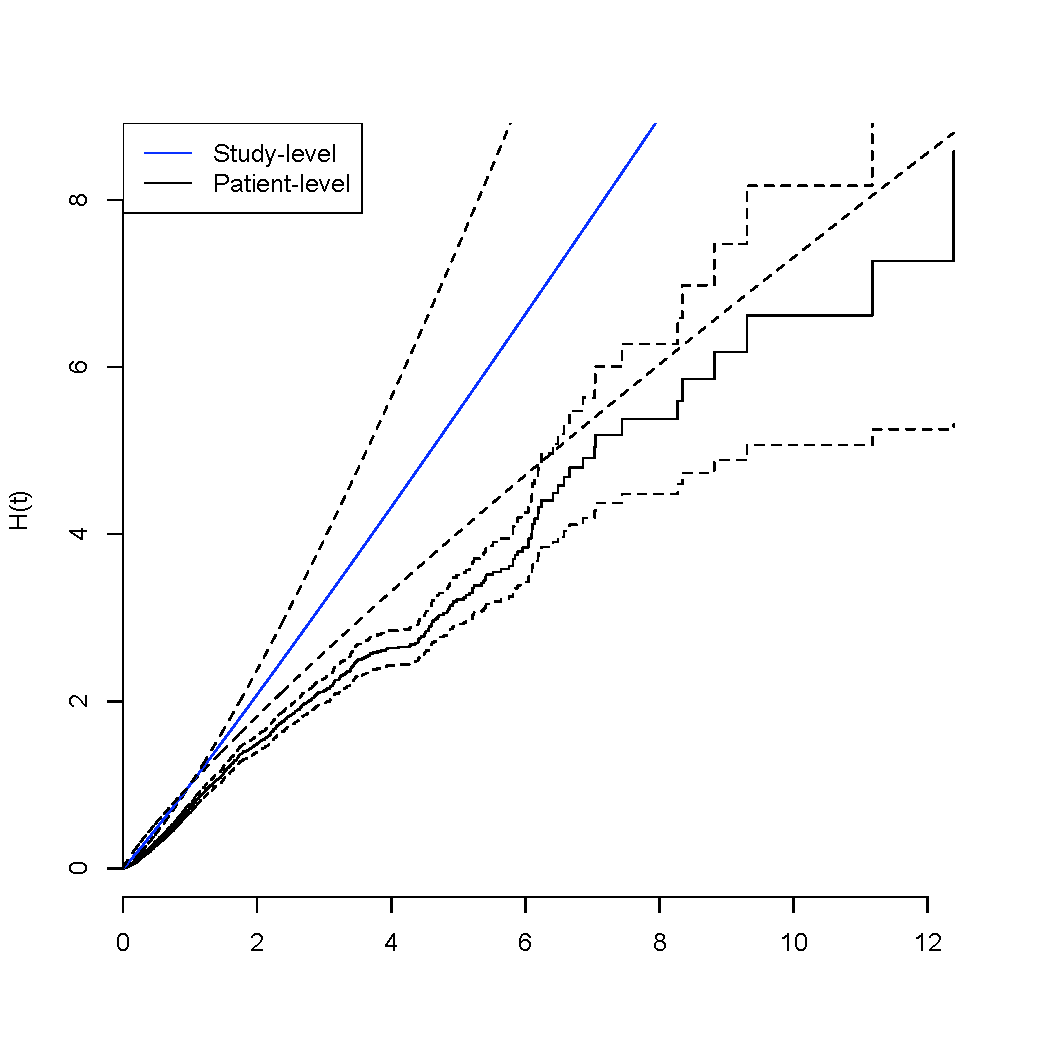
\includegraphics{haz.pdf}
\caption{Baseline hazard estimated by study-level and patient-level
  models of mixed-level meta-analysis. Dotted lines denote the 95\% CI.}
\end{figure}

\clearpage

\label{ref:ref}

\bibliographystyle{wileyj}

\bibliography{/Users/skoval/meta/bib/survival,/Users/skoval/meta/bib/survival.meta,/Users/skoval/meta/bib/statistics,/Users/skoval/meta/bib/meta,/Users/skoval/meta/bib/ecological_bias,/Users/skoval/meta/bib/likelihood,/Users/skoval/meta/bib/bayes.meta,/Users/skoval/meta/bib/bayes,/Users/skoval/meta/bib/power_loss,/Users/skoval/meta/bib/cox_randomeffects,/Users/skoval/meta/bib/importance_sampling,/Users/skoval/bibliography/public_health,/Users/skoval/bibliography/cer,/Users/skoval/meta/bib/bhits}


\end{document}


\clearpage

\section{Estimation for Cox Mixed Effects Model: coxmcem}

\subsection{Description}

The Cox mixed effects model is an extension of the standard Cox
regression model for censored data \cite{Cox1972a,Cox1975a}. It
suitable for censored data where the unit of analysis is clustered in
some way, for example, children within households. It builds on
frailty models by allowing for more complex random effects structures
corresponding to more complex grouping, for example, twins among
siblings within household. The general framework has also been
described as a proportional hazards mixed model or multivariate
frailty model. 

Estimation approaches have included approximate and sampling
methods. Approximate methods are based on a Laplace approximation to
the marginal log-likelihood \cite{Ripatti2000a}. This is implemented
by the package \texttt{coxme} of Therneau \cite{Therneau2009a}. It is well-known that the
loss of information with the approximation results in an
underestimation of the parameter standard errors \cite{Abrahantes2007a}.

Sampling methods take an expectation-maximization approach which has
the advantage of retaining all information on the model
parameters. Sampling is required at the E-step. Vaida and Xu (2000) propose
a Gibbs adaptive rejection sampling method to sample the posterior
frailties given a multivariate-normal prior \cite{Vaida2000a}. This
approach is implemented with the package \texttt{phmm}
\cite{Donohue2010a}. Ripatti, Larsen and Palmgren (2002) suggest a rejection sampler; the author is not
aware of any software for this strategy \cite{Ripatti2002a}. The difficulty
with sampling approaches is that convergence has to be checked at the
E-step and is a challenge to automate. 

The \texttt{coxmcem} uses importance sampling to obtain averages for
the multivariate frailties at the E-step. Booth and Hobert (1999) give a description of
the general approach for generalized linear mixed models
\cite{Booth1999a}. The appeal of an importance-sample is that it obviates the need for
convergence to the target distribution while retaining all information
about the model parameters. The proposal density for the
\texttt{coxmcem} implementation is a
multivariate T whose location is the maximum-likelihood estimate of
the frailties at the current EM iteration. Monitoring the MC error and
parameter estimates follows the procedure outlined by Ripatti~\emph{et
  al.} (2002). 


\subsection{Usage}

I illustrate the use of \texttt{coxmcem}. An often used test case for
frailty models is a data set of time to tumor occurrence for 50 litters of
rats \cite[chapter 9]{Therneau2000a}, with one of three rats in each litter randomly selected to recieve
a
carcinogen exposure \citep{Mantel1977a}. This is the data that will be
used for the case study. The first few rows are given below

\begin{Schunk}
\begin{Sinput}
library(ipdmeta)
data(cancer.rats)
head(cancer.rats)
  litter rx time event
1      1  1  101      0
2      1  0   49      1
3      1  0  104      0
4      2  1  104      0
5      2  0  102      0
6      2  0  104      0
\end{Sinput}
\end{Schunk}

\subsubsection{Model}

The PHMM model for time-to-tumor occurence for the
\texttt{cancer.rats} data is

\begin{equation}
\label{eq:uni}
\lambda(t) = \lambda_0(t) \mbox{exp}\lbrace x_{rx,i} \beta + b_{k(i)} \rbrace
\end{equation}

\noindent where $x_{rx,i}$ is the ith rat's indicator for carcinogen
exposure and $b_k$ is the kth litter frailty with ith subject litter
membership k(i). All K = 50 frailties share the normal distribution $b_k \sim N(0,\sigma^2)$. 

\subsubsection{Implementation}

PHMM (\ref{eq:uni}) with importance sampling is implemented as follows

\begin{Schunk}
\begin{Sinput}
set.seed(123321)

fit <- coxmcem(
    Surv(time,event)~rx,
    random=~(1|litter),
    n.groups=50,
    data=cancer.rats,
    max.iter=20,
    min.sample=500,
    mc.step=2,
    est.delta=1/100,
    df=30
)
\end{Sinput}
\end{Schunk}

The formula for the survival object is the same as would be supplied
to any of the models of \texttt{survival}. The random formula
indicated the frailty structure. Here I specifiy a baseline frailty
by litter. The number of groups is the number of clusters in the data
set. In this case clustering is by litter and there are 50 total
litters. Next, I indicate the name of the data frame containing the
variables described in the model formulas.

The remaining arguments determine the stopping rule for the EM
importance sampling procedure. The argument \texttt{min.sample}
indicates the number of draws from the joint T distribution for the
frailties that are generated at each E step. The sample determines the
number of frailties in the Monte Carlo estimate of the averages for
the complete log-likelihood. It is typical to begin with a small
number while the model estimates are far from the MLE and increase the
sample with the algorithm iterations. In this case I specify a
starting sample size of 1000. Because the algorithm will run more
slowly with a larger sample size, it is best to begin with a small
number, say 200, if suitable choices for some of the arguments,
i.e. \texttt{df}, are still being worked out.

Convergence of the algorithm is judged by the relative change of the
model paramters. Denote the set of fixed effects and frailty variance
parameters as $\theta$. In this example $\theta$ consists of the fixed
effects estimate for the treatment effect \texttt{rx} and univariate
frailty variance $\texttt{vcov} = \sigma^2$. The relative change in each parameter from the
previous iteration is determined. If the maximum change among all
parameters is less than \texttt{est.delta}, \emph{for three
  consecutive iterations}, then the algorithm
stops. With a setting for \texttt{est.delta} of $\frac{1}{100}$ this
would mean that a less than 1\% relative change for all parameters is
required for three iterations in a row in order to stop. For this
reason, the minimum number of iterations for any implementation is three.

If \texttt{max.iter} is reached before the convergence threshold has
been met, the algorithm stops.

The argument \texttt{mc.step} determines how the E-step frailty sample
size is increased. When the coefficient of variation of the relative
change of the parameters is large, this suggests that the MC error is
too large and the sample size should be increased. Thus, when the
three most recent relative change between consecutive EM estimates
have a coefficient of variation greater than unity, the current sample
size of N is increased by 

\[
N = N + \frac{1}{\mbox{mc.step}}N
\]


\subsubsection{Summary}

First I review the algorithm properties to see if enough iterations
and MC samples have been obtained. 

\begin{Schunk}
\begin{Sinput}
fit[1:5]
$max.weight
[1] 0.01193944 0.01176729 0.01087182

$mc.samples
[1] 500 500 500

$est.converge
[1] 0.006424424 0.009711094 0.001660967

$loglik
[1] -177.5236 -177.7699 -177.8148

$sd.loglik
[1] 9.276321 8.759723 8.369623
\end{Sinput}
\end{Schunk}

The algorithm stopped after 3 iterations, the minimum possible, so
that the MC sample size never exceeded the initial starting value. The
maximum weights are the maximum weights among all importance weights
for the given iteration. These will each be a value between (0,1)
since the sum of all importance weights are 1, their being
normalized. For a sample size of N, each iteration draws N joint
frailties, in this case 500 vectors of 50 frailties. Averages of the frailties are
the importance-weighted average of the N-size sample. No single set of
frailties should dominate this average so it needs to be checked that
the weights are fairly evenly distributed. If the weights were all
equal, each would be $\frac{1}{N}$. A maximum weight much greater than
this would suggest that some adjustments were needed in the model of T
proposal distribution settings. Here I see that no single draw
contributed greater than approximately 1\% to the average so the
algorithm settings seem to be fine.

The standard deviation of the log-likelihood can complement the
interpretation of the importance weights. These are the standard
deviations of the conditional log-likelihood of the PHMM conditional
on each
sample frailty of the given iteration. There should be enough
variation in the frailties to be sure that the full support is
represented. However, large variation could produce great imbalances
in the importance weights. So if the \texttt{max.weights} seem large, and the
standard deviation of the log-likelihoods are large relative to the
MLE log-likelihood values, this would suggest that the T proposal
settings need to be modified or that the model has been poorly
specified. For example, one way to reduce variation in the frailty
proposal would be to lower the \texttt{df}. In general, a good
starting place might be to set \texttt{df} to the number of clusters
in the data set, approximately.

Regarding the model estimates, I find that the final iteration
stopped with a relative maximal change of 0.17\%, meaning that both
the \texttt{coef} and \texttt{vcov} estimates had less than 0.2\% change
from the previous iteration values. By specifying a \texttt{est.delta}
of 1\%, I required that the algorithm proceed until three consecutive
relative changes had maximum differences of 1\% or less. This was met
after the minimum three iterations in this case.

Being satisfied with the convergence properties of the MCEM I now
consider the findings. The fixed effect estimates are the list element \texttt{coef} and the
frailty variance parameters \texttt{vcov}.

\begin{Schunk}
\begin{Sinput}
> fit$coef
      rx 
0.910061 

> fit$vcov
          [,1]
[1,] 0.4316714
\end{Sinput}
\end{Schunk}

Variances for each of these parameters are contained in the list
\texttt{var}. A large-sample 95\% CI for the hazard ratio
of tumor occurrence given carcinogen exposure can be obtained with the
following code. I show the do-it-yourself way then a version which
makes  use of the confidence interval function \texttt{ci}.

\begin{Schunk}
\begin{Sinput}
> exp(fit$coef+c(-2,2)*sqrt(fit$var$coef))
[1] 1.300951 4.744692

> ci(1,fit$coef,fit$var$coef)
      low point.est      high 
 1.317909  2.484474  4.683640 
\end{Sinput}
\end{Schunk}

The interpretation is that there is a 2.5 increased risk to developing
a tumor for rats exposed to the carcinogen which can be stated with
95\% confidence.

The variability between litters in baseline risk was

\begin{Schunk}
\begin{Sinput}
sqrt(fit$vcov)
         [,1]
[1,] 0.657017

> ci(1,0,fit$vcov,alpha=.3)
      low point.est      high 
0.5061337 1.0000000 1.9757625 
\end{Sinput}
\end{Schunk}

\noindent suggesting that there is a roughly 30\% chance that
otherwise equivalent rats with respect to exposure could have a
relative hazard outside of the interval (0.51, 1.98), with 30\%
probability, which seems a substantial level of heterogeneity.

A Wald test for the significance of the fixed effects can be obtained
by computing the Wald test-statistics using the variances of the
\texttt{coef}.

\begin{Schunk}
\begin{Sinput}
> fit$coef/sqrt(get.diag(fit$var$coef))
      rx 
2.813322 

> p.value <- pnorm(abs(fit$coef/sqrt(get.diag(fit$var$coef))),lower=FALSE)
> p.value
         rx 
0.002451630 
\end{Sinput}
\end{Schunk}

Testing of the random effect is more challenging because of the
asymptotic properties of common tests when the variance parameter is
near the boundary, that is, the null hypothesis that the variance is
zero. A Wald test can be a useful exploratory tool but a likelihood
ratio test is generally preferred \cite{Self1987a}.

\begin{Schunk}
\begin{Sinput}
> fit$vcov/sqrt(fit$var$vcov)
         [,1]
[1,] 1.868417
\end{Sinput}
\end{Schunk}

This gives support for the inclusion of the baseline litter random
effect. 

\subsubsection{Recognizing a Poorly Specified Model}

I now consider how to identify a poorly fit model when the random
effect and fixed effects structures have been misspecified. I do this
be introducing an unrelated variable into the model. The `noise' term
is included as a fixed and random effect.

\begin{equation}
\label{eq:uni}
\lambda(t) = \lambda_0(t) \mbox{exp}\lbrace x_{rx,i} \beta_1 +
x_{noise,i} \beta_2 + b_{k(i),1} +  b_{k(i),2} x_{noise,i} \rbrace
\end{equation}

\noindent with 

\[
\begin{pmatrix} b_{k,1} \\ b_{k,2} \end{pmatrix} \sim
MVN(\mathbf{0},\begin{pmatrix} \theta_1 & \theta_3 \\
\theta_3 & \theta_2 \end{pmatrix})
\]

\noindent And the implemenation is given by 

\begin{Schunk}
\begin{Sinput}
set.seed(456654)

cancer.rats$noise <- runif(150)

fit <- coxmcem(
    Surv(time,event)~rx+noise,
    random=~(1+noise|litter),
    n.groups=50,
    data=cancer.rats,
    max.iter=10,
    min.sample=300,
    mc.step=2,
    est.delta=1/100,
    df=30
)
\end{Sinput}
\end{Schunk}

Since I am initially unsure about the fit of this model, I do a
trial run with a smaller initial sample size and fewer
iterations. Monitoring the relative change in estimates I note some
cases of high change. One way in which this could occur is when a
parameter of the model is close to zero, so that small absolute
changes in estimates result in large relative changes.

I also note some iterations with high \texttt{max.weight} and
\texttt{sd.loglik}. Looking at the fixed effect estimates, I conclude
that the \texttt{noise} term is not contributing any information to the
tumor-occurrence outcome and that the large relative changes in the
parameters (large \texttt{est.delta}) was due to the noise coefficient
being near to zero.

\begin{Schunk}
\begin{Sinput}
> fit$coef/sqrt(get.diag(fit$var$coef))
      rx    noise 
3.019627 0.642682 
\end{Sinput}
\end{Schunk}


\section{Mixed-level Meta-analysis: mlma}

Mixed-level meta-analysis (MLMA) describes a quantitative summary of
evidence at disparate levels with some trials providing
individual-level data and other trials summary data. The \texttt{mlma}
function performs MLMA estimation when the outcome is a time-to-event
and aggregate data is in the form of a set of survival estimates
within treatment group, within study. 

The individual patient data (IPD) model is a proportional hazards
mixed model (PHMM) allowing a general random effects structure with multivariate normal
frailties. The study-level model is a multivariate mixed model on the
complementary-log-log of the study-specific survival estimates. This
study-level model is the implied linear relation based on the
assumption that all outcomes follow the PHMM at the patient level. 

Through
combined likelihood maximization, both evidence levels contribute to
the estimation of shared fixed effects and the frailty variance
structures. The estimation uses an MCEM approach with importance
sampling following the same procedure are for the PHMM analysis
implemented by \texttt{coxmcem}. Separation of the patient-level and study-level effects is
also possible if there is concern of non-equivalence in the risk
associations at the aggregate level versus the subject level.

\subsection{Usage}

Consider a mixed-level dataset consisting of 8 IPD and 2
study-level RCTs. The model for the PHMM has treatment main effect. A bivariate frailty
for baseline and treatment effect by trial is the random component.

See \texttt{example(ipd.data)} and \texttt{example(meta.data)} for a
quick visual display of the nature of the mixed-level data for this
example.

To obtain the MLMA estimates, I specify model formula for the study- and
individual-level models. The individual-level model is a hazard-based
model and takes a formula like that for \texttt{survfit} or \texttt{coxph}.
The study-level model is based on aggregated survival proportions with
their squared standard errors (\texttt{sigma2}). The random component
uses indicated the frailty structure using the same form as for
\texttt{coxme} or \texttt{lme}. The argument
\texttt{study.group.interaction} is the factor that is the
cluster, here \texttt{group}, and the treatment group indicator. This
factor identifies the membership to the within treatment, within study
groups for which separate survival estimates have been collected. 

To gain some guidance in selection of the fixed effects model I can
make use of a less computationally intense analysis with the patient-level data. 

\begin{Schunk}
\begin{Sinput}
> fit.coxph <- coxph(Surv(time,event)~trt*x,ipd.data)
> fit.coxph
Call:
coxph(formula = Surv(time, event) ~ trt * x, data = ipd.data)


          coef exp(coef) se(coef)      z       p
trt   -0.45666     0.633   0.0583 -7.832 4.8e-15
x      0.02494     1.025   0.0291  0.856 3.9e-01
trt:x -0.00906     0.991   0.0419 -0.216 8.3e-01

Likelihood ratio test=70.3  on 3 df, p=3.66e-15  n= 1600 
\end{Sinput}
\end{Schunk}

This suggests that the candidate covariate is not important. I can
verify this with a trial run of \texttt{mlma}. The model components are
as follows.

The patient-level PHMM model is

\[
\lambda_i(t|b) = \lambda_0(t) \mbox{exp}\lbrace x_{trt,i} \beta_1 +
x_i \beta_2 + b_{k(i),1} + b_{k(i),2} x_{trt,i} \rbrace
\]

\noindent where k(i) is the study membership for the ith subject. Each
$b_k$ is a bivariate normal frailty with general variance structure.

The study-level model for each KM survival estimate provided by study
is

\[
g(s_i|\tilde{b}) = \mbox{log}(t_i) + \tilde{x}_{trt,i} \beta_1 +
\tilde{x}_i \beta_2 + \tilde{b}_{j(i)}+\tilde{b}_{j(i),2} \tilde{x}_{trt,i} +\epsilon_i
\]

\noindent Here $g(x) = log(-log(x))$  and $\epsilon_i \sim
N(0,\sigma_i^2)$ where $\sigma_i^2$ is considered known. The residual
variance is determined by the standard error for the KM estimate and
applying the delta method for the complementary-log-log
transform. When there are multiple estimates from the same study, the
variance structure accounts for correlation within treatment group,
within trial. The methodology is in keeping with \cite{Arends2008a}.

The covariates for the study-level model are grouped which is why I
have used the notation $\tilde{x}$ to distinguish them from the
patient-level model. Thus, the patient level factor $x$ when
aggregated into the cluster sample means is denoted as $\tilde{x}$.

Implementation of the model proceeds as follows:

\begin{Schunk}
\begin{Sinput}
set.seed(123321)
data(ipd.data)
data(meta.data)

fit <- mlma(
    Surv(time,event)~trt+x,
    surv~-1+log(time)+trt+x,
    random=~(1+trt|group),
    ipd.groups=8,
    meta.groups=2,
    ipd.data=ipd.data,
    meta.data=meta.data,
    sigma2=meta.data$sigma2,
    study.group=meta.data$sub.group,
    max.iter=10,
    est.delta=.01,
    min=300
)

> #WALD TEST FOR FIXED EFFECTS
> fit$coef
        trt           x   log(time) 
-0.63023004  0.00326478  1.04518270 

> fit$coef/sqrt(diag(fit$var$coef))
        trt           x   log(time) 
-6.45590592  0.09845826 10.47860368 

> sqrt(fit$vcov)
          [,1]      [,2]
[1,] 0.6430685 0.3374159
[2,] 0.3374159 0.3759782
> 

> #WALD TEST FOR FRAILTY VARIANCES
> sqrt(diag(fit$vcov))
[1] 0.6430685 0.3759782
> diag(fit$vcov)/sqrt(fit$var$vcov)
         [,1]
[1,] 2.062913
[2,] 1.849326
\end{Sinput}
\end{Schunk}

There is no evidence of a significant effect for the covariate
\texttt{x} so I remove this factor and re-fit with just the treatment
effect. I examine the estimates with the revised fit.

\begin{Schunk}
\begin{Sinput}
> fit$coef
       trt  log(time) 
-0.5352532  1.0558993 

> fit$coef/sqrt(diag(fit$var$coef))
      trt log(time) 
-6.125604 10.800622 
> sqrt(diag(fit$vcov))
[1] 0.6342262 0.3850056
> diag(fit$vcov)/sqrt(fit$var$vcov)
         [,1]
[1,] 2.067657
[2,] 1.987731
\end{Sinput}
\end{Schunk}

All of the model parameters contribute important information to
survival outcomes. 

\begin{Schunk}
\begin{Sinput}
> fit$est.con[(fit$iter-5):fit$iter]
[1] 0.09792774 0.09908291 0.06861460 0.07117281 0.05336713 0.12839772
\end{Sinput}
\end{Schunk}

The convergence criterion was not met, however, so I will want to
adjust the number of MC samples of the number of iterations before
drawing firm conclusions from \texttt{fit}.

When the converged estimates have been obtained I can compare the
baseline hazard implied by each model, which is another check of the
consistency between the patient-level and study-level data (Figure 1).

\begin{Schunk}
\begin{Sinput}
H <- bas.haz(
             Surv(time,event)~trt,
             ~-1+log(t),
             ipd.data,
             fit$coef,
             fit$var$coef,
             )

#PATIENT-LEVEL BASELINE HAZARD

plot(H$ipd.survfit,fun="cumhaz",ylab="H(t)",bty="n")

#STUDY-LEVEL BASELINE HAZARD WITH 95\% CI

lines(x=H$meta.bas.haz$time,y=H$meta.bas.haz$lower,type="l",lty=2)
lines(x=H$meta.bas.haz$time,y=H$meta.bas.haz$est,type="l",col="blue")
lines(x=H$meta.bas.haz$time,y=H$meta.bas.haz$upper,type="l",lty=2)

legend("topleft",legend=c("Study-level","Patient-level"),lty=1,col=c("blue","black"))
\end{Sinput}
\end{Schunk}

If a fixed effects model was wanted, I can obtain it through the
\texttt{fixed} argument.

\begin{Schunk}
\begin{Sinput}
fit.fixed <- mlma(
    Surv(time,event)~trt,
    surv~-1+log(time)+trt,
    random=~(1+trt|group),
    ipd.groups=8,
    meta.groups=2,
    ipd.data=ipd.data,
    meta.data=meta.data,
    sigma2=meta.data$sigma2,
    study.group=meta.data$sub.group,
    fixed=TRUE
)

> fit.fixed$coef
      trt log(time) 
-0.476680  1.127154 
\end{Sinput}
\end{Schunk}

This provides a means of constructing a likelihood ratio test for the
frailty variances, compared the fixed effects model likelihood to the
mixed effects model. 

\begin{Schunk}
\begin{Sinput}
> #LIKELIHOOD RATIO TEST STATISTIC
> -2*(fit.fixed$loglik-fit$loglik[fit$iter])
         [,1]
[1,] 659.4629
\end{Sinput}
\end{Schunk}

Comparing this statistic to a $\chi^2(3)$ for the 3 variance parameters of the
general covariance-variance structure for the frailties of the mixed
model gives some guidance on the presence of significant intercluster
variation. In this case, there is strong evidence of heterogeneity
among outcomes.

\subsection{Ecological Bias}

If I were concerned that my conclusions about the covariate \texttt{x}
were mislead by the presence of a study-level bias, I can separate
the parameterization for each evidence-level. I do this by
introducing a centered covariate into the individual level model. Note
that the model formulae have to have the same term label for all
shared effects.

The patient-level PHMM model changes to

\[
\lambda_i(t|b) = \lambda_0(t) \mbox{exp}\lbrace x_{trt,i} \beta_1 +
(x_i - x_i^{*}) \beta_2 + x_i^{*} \beta_3 + b_{k(i),1} + b_{k(i),2} x_{trt,i} \rbrace
\]

\noindent where $x_i^{*}$ is the k(i) sample average of the covariate,
the grouped effect. Thus, $\beta_2$ is the patient-level effect while
$\beta_3$ is the study-level effect. Accordingly, the study-level
model is

\[
g(s_i|\tilde{b}) = \mbox{log}(t_i) + \tilde{x}_{trt,i} \beta_1 +
\tilde{x}_i^{*} \beta_3 + \tilde{b}_{j(i),1}+\tilde{b}_{j(i),2} \tilde{x}_{trt,i} +\epsilon_i
\]

\noindent where the notation of the covariate has changed to
correspond with the patient-level model, but the elements are still
the study-level sample averages for the covariate \texttt{x}.

\begin{Schunk}
\begin{Sinput}
n <- table(ipd.data$group)
ipd.data$x.star <- rep(tapply(ipd.data$x,ipd.data$group,mean),n)
names(meta.data)[which(names(meta.data)=="x")] <- "x.star"

fit.bias <- mlma(
    Surv(time,event)~trt+I(x-x.star)+x.star,
    surv~-1+log(time)+trt+x.star,
    random=~(1+trt|group),
    ipd.groups=8,
    meta.groups=2,
    ipd.data=ipd.data,
    meta.data=meta.data,
    sigma2=meta.data$sigma2,
    study.group=meta.data$sub.group,
    max.iter=20,mc=1.3,
    est.delta=.01,
    df=25,
    min=500
)

> fit.bias$coef
          trt I(x - x.star)        x.star     log(time) 
 -0.553248425   0.006493564   0.306708999   1.073181569 

> ci(c(0,-1,1,0),fit.bias$coef,fit.bias$var$coef,f=function(x){x})
      low point.est      high 
0.2795519 0.3002154 0.3208790 
\end{Sinput}
\end{Schunk}

I obtain the 95\% CI for the contrast between the study- and
patient-level effect for the covariate \texttt{x.star}. There is evidence
that a positive relation at the study-level is present, while no
individual-level relation is demonstrated.


\clearpage

\begin{figure}\center
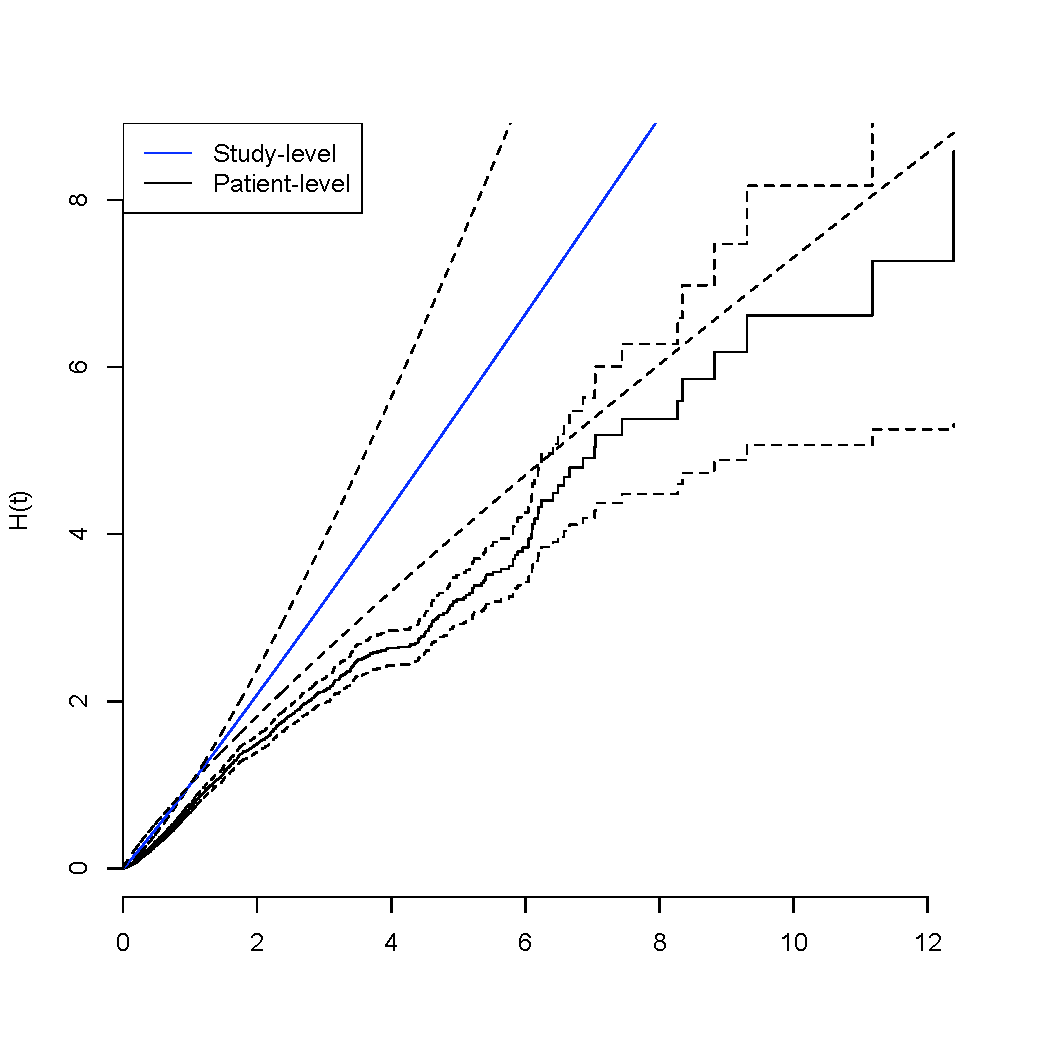
\includegraphics{haz.pdf}
\caption{Baseline hazard estimated by study-level and patient-level
  models of mixed-level meta-analysis. Dotted lines denote the 95\% CI.}
\end{figure}

\clearpage

\label{ref:ref}

\bibliographystyle{wileyj}

\bibliography{/Users/skoval/meta/bib/survival,/Users/skoval/meta/bib/survival.meta,/Users/skoval/meta/bib/statistics,/Users/skoval/meta/bib/meta,/Users/skoval/meta/bib/ecological_bias,/Users/skoval/meta/bib/likelihood,/Users/skoval/meta/bib/bayes.meta,/Users/skoval/meta/bib/bayes,/Users/skoval/meta/bib/power_loss,/Users/skoval/meta/bib/cox_randomeffects,/Users/skoval/meta/bib/importance_sampling,/Users/skoval/bibliography/public_health,/Users/skoval/bibliography/cer,/Users/skoval/meta/bib/bhits}


\end{document}


\clearpage

\section{Estimation for Cox Mixed Effects Model: coxmcem}

\subsection{Description}

The Cox mixed effects model is an extension of the standard Cox
regression model for censored data \cite{Cox1972a,Cox1975a}. It
suitable for censored data where the unit of analysis is clustered in
some way, for example, children within households. It builds on
frailty models by allowing for more complex random effects structures
corresponding to more complex grouping, for example, twins among
siblings within household. The general framework has also been
described as a proportional hazards mixed model or multivariate
frailty model. 

Estimation approaches have included approximate and sampling
methods. Approximate methods are based on a Laplace approximation to
the marginal log-likelihood \cite{Ripatti2000a}. This is implemented
by the package \texttt{coxme} of Therneau \cite{Therneau2009a}. It is well-known that the
loss of information with the approximation results in an
underestimation of the parameter standard errors \cite{Abrahantes2007a}.

Sampling methods take an expectation-maximization approach which has
the advantage of retaining all information on the model
parameters. Sampling is required at the E-step. Vaida and Xu (2000) propose
a Gibbs adaptive rejection sampling method to sample the posterior
frailties given a multivariate-normal prior \cite{Vaida2000a}. This
approach is implemented with the package \texttt{phmm}
\cite{Donohue2010a}. Ripatti, Larsen and Palmgren (2002) suggest a rejection sampler; the author is not
aware of any software for this strategy \cite{Ripatti2002a}. The difficulty
with sampling approaches is that convergence has to be checked at the
E-step and is a challenge to automate. 

The \texttt{coxmcem} uses importance sampling to obtain averages for
the multivariate frailties at the E-step. Booth and Hobert (1999) give a description of
the general approach for generalized linear mixed models
\cite{Booth1999a}. The appeal of an importance-sample is that it obviates the need for
convergence to the target distribution while retaining all information
about the model parameters. The proposal density for the
\texttt{coxmcem} implementation is a
multivariate T whose location is the maximum-likelihood estimate of
the frailties at the current EM iteration. Monitoring the MC error and
parameter estimates follows the procedure outlined by Ripatti~\emph{et
  al.} (2002). 


\subsection{Usage}

I illustrate the use of \texttt{coxmcem}. An often used test case for
frailty models is a data set of time to tumor occurrence for 50 litters of
rats \cite[chapter 9]{Therneau2000a}, with one of three rats in each litter randomly selected to recieve
a
carcinogen exposure \citep{Mantel1977a}. This is the data that will be
used for the case study. The first few rows are given below

\begin{Schunk}
\begin{Sinput}
library(ipdmeta)
data(cancer.rats)
head(cancer.rats)
  litter rx time event
1      1  1  101      0
2      1  0   49      1
3      1  0  104      0
4      2  1  104      0
5      2  0  102      0
6      2  0  104      0
\end{Sinput}
\end{Schunk}

\subsubsection{Model}

The PHMM model for time-to-tumor occurence for the
\texttt{cancer.rats} data is

\begin{equation}
\label{eq:uni}
\lambda(t) = \lambda_0(t) \mbox{exp}\lbrace x_{rx,i} \beta + b_{k(i)} \rbrace
\end{equation}

\noindent where $x_{rx,i}$ is the ith rat's indicator for carcinogen
exposure and $b_k$ is the kth litter frailty with ith subject litter
membership k(i). All K = 50 frailties share the normal distribution $b_k \sim N(0,\sigma^2)$. 

\subsubsection{Implementation}

PHMM (\ref{eq:uni}) with importance sampling is implemented as follows

\begin{Schunk}
\begin{Sinput}
set.seed(123321)

fit <- coxmcem(
    Surv(time,event)~rx,
    random=~(1|litter),
    n.groups=50,
    data=cancer.rats,
    max.iter=20,
    min.sample=500,
    mc.step=2,
    est.delta=1/100,
    df=30
)
\end{Sinput}
\end{Schunk}

The formula for the survival object is the same as would be supplied
to any of the models of \texttt{survival}. The random formula
indicated the frailty structure. Here I specifiy a baseline frailty
by litter. The number of groups is the number of clusters in the data
set. In this case clustering is by litter and there are 50 total
litters. Next, I indicate the name of the data frame containing the
variables described in the model formulas.

The remaining arguments determine the stopping rule for the EM
importance sampling procedure. The argument \texttt{min.sample}
indicates the number of draws from the joint T distribution for the
frailties that are generated at each E step. The sample determines the
number of frailties in the Monte Carlo estimate of the averages for
the complete log-likelihood. It is typical to begin with a small
number while the model estimates are far from the MLE and increase the
sample with the algorithm iterations. In this case I specify a
starting sample size of 1000. Because the algorithm will run more
slowly with a larger sample size, it is best to begin with a small
number, say 200, if suitable choices for some of the arguments,
i.e. \texttt{df}, are still being worked out.

Convergence of the algorithm is judged by the relative change of the
model paramters. Denote the set of fixed effects and frailty variance
parameters as $\theta$. In this example $\theta$ consists of the fixed
effects estimate for the treatment effect \texttt{rx} and univariate
frailty variance $\texttt{vcov} = \sigma^2$. The relative change in each parameter from the
previous iteration is determined. If the maximum change among all
parameters is less than \texttt{est.delta}, \emph{for three
  consecutive iterations}, then the algorithm
stops. With a setting for \texttt{est.delta} of $\frac{1}{100}$ this
would mean that a less than 1\% relative change for all parameters is
required for three iterations in a row in order to stop. For this
reason, the minimum number of iterations for any implementation is three.

If \texttt{max.iter} is reached before the convergence threshold has
been met, the algorithm stops.

The argument \texttt{mc.step} determines how the E-step frailty sample
size is increased. When the coefficient of variation of the relative
change of the parameters is large, this suggests that the MC error is
too large and the sample size should be increased. Thus, when the
three most recent relative change between consecutive EM estimates
have a coefficient of variation greater than unity, the current sample
size of N is increased by 

\[
N = N + \frac{1}{\mbox{mc.step}}N
\]


\subsubsection{Summary}

First I review the algorithm properties to see if enough iterations
and MC samples have been obtained. 

\begin{Schunk}
\begin{Sinput}
fit[1:5]
$max.weight
[1] 0.01193944 0.01176729 0.01087182

$mc.samples
[1] 500 500 500

$est.converge
[1] 0.006424424 0.009711094 0.001660967

$loglik
[1] -177.5236 -177.7699 -177.8148

$sd.loglik
[1] 9.276321 8.759723 8.369623
\end{Sinput}
\end{Schunk}

The algorithm stopped after 3 iterations, the minimum possible, so
that the MC sample size never exceeded the initial starting value. The
maximum weights are the maximum weights among all importance weights
for the given iteration. These will each be a value between (0,1)
since the sum of all importance weights are 1, their being
normalized. For a sample size of N, each iteration draws N joint
frailties, in this case 500 vectors of 50 frailties. Averages of the frailties are
the importance-weighted average of the N-size sample. No single set of
frailties should dominate this average so it needs to be checked that
the weights are fairly evenly distributed. If the weights were all
equal, each would be $\frac{1}{N}$. A maximum weight much greater than
this would suggest that some adjustments were needed in the model of T
proposal distribution settings. Here I see that no single draw
contributed greater than approximately 1\% to the average so the
algorithm settings seem to be fine.

The standard deviation of the log-likelihood can complement the
interpretation of the importance weights. These are the standard
deviations of the conditional log-likelihood of the PHMM conditional
on each
sample frailty of the given iteration. There should be enough
variation in the frailties to be sure that the full support is
represented. However, large variation could produce great imbalances
in the importance weights. So if the \texttt{max.weights} seem large, and the
standard deviation of the log-likelihoods are large relative to the
MLE log-likelihood values, this would suggest that the T proposal
settings need to be modified or that the model has been poorly
specified. For example, one way to reduce variation in the frailty
proposal would be to lower the \texttt{df}. In general, a good
starting place might be to set \texttt{df} to the number of clusters
in the data set, approximately.

Regarding the model estimates, I find that the final iteration
stopped with a relative maximal change of 0.17\%, meaning that both
the \texttt{coef} and \texttt{vcov} estimates had less than 0.2\% change
from the previous iteration values. By specifying a \texttt{est.delta}
of 1\%, I required that the algorithm proceed until three consecutive
relative changes had maximum differences of 1\% or less. This was met
after the minimum three iterations in this case.

Being satisfied with the convergence properties of the MCEM I now
consider the findings. The fixed effect estimates are the list element \texttt{coef} and the
frailty variance parameters \texttt{vcov}.

\begin{Schunk}
\begin{Sinput}
> fit$coef
      rx 
0.910061 

> fit$vcov
          [,1]
[1,] 0.4316714
\end{Sinput}
\end{Schunk}

Variances for each of these parameters are contained in the list
\texttt{var}. A large-sample 95\% CI for the hazard ratio
of tumor occurrence given carcinogen exposure can be obtained with the
following code. I show the do-it-yourself way then a version which
makes  use of the confidence interval function \texttt{ci}.

\begin{Schunk}
\begin{Sinput}
> exp(fit$coef+c(-2,2)*sqrt(fit$var$coef))
[1] 1.300951 4.744692

> ci(1,fit$coef,fit$var$coef)
      low point.est      high 
 1.317909  2.484474  4.683640 
\end{Sinput}
\end{Schunk}

The interpretation is that there is a 2.5 increased risk to developing
a tumor for rats exposed to the carcinogen which can be stated with
95\% confidence.

The variability between litters in baseline risk was

\begin{Schunk}
\begin{Sinput}
sqrt(fit$vcov)
         [,1]
[1,] 0.657017

> ci(1,0,fit$vcov,alpha=.3)
      low point.est      high 
0.5061337 1.0000000 1.9757625 
\end{Sinput}
\end{Schunk}

\noindent suggesting that there is a roughly 30\% chance that
otherwise equivalent rats with respect to exposure could have a
relative hazard outside of the interval (0.51, 1.98), with 30\%
probability, which seems a substantial level of heterogeneity.

A Wald test for the significance of the fixed effects can be obtained
by computing the Wald test-statistics using the variances of the
\texttt{coef}.

\begin{Schunk}
\begin{Sinput}
> fit$coef/sqrt(get.diag(fit$var$coef))
      rx 
2.813322 

> p.value <- pnorm(abs(fit$coef/sqrt(get.diag(fit$var$coef))),lower=FALSE)
> p.value
         rx 
0.002451630 
\end{Sinput}
\end{Schunk}

Testing of the random effect is more challenging because of the
asymptotic properties of common tests when the variance parameter is
near the boundary, that is, the null hypothesis that the variance is
zero. A Wald test can be a useful exploratory tool but a likelihood
ratio test is generally preferred \cite{Self1987a}.

\begin{Schunk}
\begin{Sinput}
> fit$vcov/sqrt(fit$var$vcov)
         [,1]
[1,] 1.868417
\end{Sinput}
\end{Schunk}

This gives support for the inclusion of the baseline litter random
effect. 

\subsubsection{Recognizing a Poorly Specified Model}

I now consider how to identify a poorly fit model when the random
effect and fixed effects structures have been misspecified. I do this
be introducing an unrelated variable into the model. The `noise' term
is included as a fixed and random effect.

\begin{equation}
\label{eq:uni}
\lambda(t) = \lambda_0(t) \mbox{exp}\lbrace x_{rx,i} \beta_1 +
x_{noise,i} \beta_2 + b_{k(i),1} +  b_{k(i),2} x_{noise,i} \rbrace
\end{equation}

\noindent with 

\[
\begin{pmatrix} b_{k,1} \\ b_{k,2} \end{pmatrix} \sim
MVN(\mathbf{0},\begin{pmatrix} \theta_1 & \theta_3 \\
\theta_3 & \theta_2 \end{pmatrix})
\]

\noindent And the implemenation is given by 

\begin{Schunk}
\begin{Sinput}
set.seed(456654)

cancer.rats$noise <- runif(150)

fit <- coxmcem(
    Surv(time,event)~rx+noise,
    random=~(1+noise|litter),
    n.groups=50,
    data=cancer.rats,
    max.iter=10,
    min.sample=300,
    mc.step=2,
    est.delta=1/100,
    df=30
)
\end{Sinput}
\end{Schunk}

Since I am initially unsure about the fit of this model, I do a
trial run with a smaller initial sample size and fewer
iterations. Monitoring the relative change in estimates I note some
cases of high change. One way in which this could occur is when a
parameter of the model is close to zero, so that small absolute
changes in estimates result in large relative changes.

I also note some iterations with high \texttt{max.weight} and
\texttt{sd.loglik}. Looking at the fixed effect estimates, I conclude
that the \texttt{noise} term is not contributing any information to the
tumor-occurrence outcome and that the large relative changes in the
parameters (large \texttt{est.delta}) was due to the noise coefficient
being near to zero.

\begin{Schunk}
\begin{Sinput}
> fit$coef/sqrt(get.diag(fit$var$coef))
      rx    noise 
3.019627 0.642682 
\end{Sinput}
\end{Schunk}


\section{Mixed-level Meta-analysis: mlma}

Mixed-level meta-analysis (MLMA) describes a quantitative summary of
evidence at disparate levels with some trials providing
individual-level data and other trials summary data. The \texttt{mlma}
function performs MLMA estimation when the outcome is a time-to-event
and aggregate data is in the form of a set of survival estimates
within treatment group, within study. 

The individual patient data (IPD) model is a proportional hazards
mixed model (PHMM) allowing a general random effects structure with multivariate normal
frailties. The study-level model is a multivariate mixed model on the
complementary-log-log of the study-specific survival estimates. This
study-level model is the implied linear relation based on the
assumption that all outcomes follow the PHMM at the patient level. 

Through
combined likelihood maximization, both evidence levels contribute to
the estimation of shared fixed effects and the frailty variance
structures. The estimation uses an MCEM approach with importance
sampling following the same procedure are for the PHMM analysis
implemented by \texttt{coxmcem}. Separation of the patient-level and study-level effects is
also possible if there is concern of non-equivalence in the risk
associations at the aggregate level versus the subject level.

\subsection{Usage}

Consider a mixed-level dataset consisting of 8 IPD and 2
study-level RCTs. The model for the PHMM has treatment main effect. A bivariate frailty
for baseline and treatment effect by trial is the random component.

See \texttt{example(ipd.data)} and \texttt{example(meta.data)} for a
quick visual display of the nature of the mixed-level data for this
example.

To obtain the MLMA estimates, I specify model formula for the study- and
individual-level models. The individual-level model is a hazard-based
model and takes a formula like that for \texttt{survfit} or \texttt{coxph}.
The study-level model is based on aggregated survival proportions with
their squared standard errors (\texttt{sigma2}). The random component
uses indicated the frailty structure using the same form as for
\texttt{coxme} or \texttt{lme}. The argument
\texttt{study.group.interaction} is the factor that is the
cluster, here \texttt{group}, and the treatment group indicator. This
factor identifies the membership to the within treatment, within study
groups for which separate survival estimates have been collected. 

To gain some guidance in selection of the fixed effects model I can
make use of a less computationally intense analysis with the patient-level data. 

\begin{Schunk}
\begin{Sinput}
> fit.coxph <- coxph(Surv(time,event)~trt*x,ipd.data)
> fit.coxph
Call:
coxph(formula = Surv(time, event) ~ trt * x, data = ipd.data)


          coef exp(coef) se(coef)      z       p
trt   -0.45666     0.633   0.0583 -7.832 4.8e-15
x      0.02494     1.025   0.0291  0.856 3.9e-01
trt:x -0.00906     0.991   0.0419 -0.216 8.3e-01

Likelihood ratio test=70.3  on 3 df, p=3.66e-15  n= 1600 
\end{Sinput}
\end{Schunk}

This suggests that the candidate covariate is not important. I can
verify this with a trial run of \texttt{mlma}. The model components are
as follows.

The patient-level PHMM model is

\[
\lambda_i(t|b) = \lambda_0(t) \mbox{exp}\lbrace x_{trt,i} \beta_1 +
x_i \beta_2 + b_{k(i),1} + b_{k(i),2} x_{trt,i} \rbrace
\]

\noindent where k(i) is the study membership for the ith subject. Each
$b_k$ is a bivariate normal frailty with general variance structure.

The study-level model for each KM survival estimate provided by study
is

\[
g(s_i|\tilde{b}) = \mbox{log}(t_i) + \tilde{x}_{trt,i} \beta_1 +
\tilde{x}_i \beta_2 + \tilde{b}_{j(i)}+\tilde{b}_{j(i),2} \tilde{x}_{trt,i} +\epsilon_i
\]

\noindent Here $g(x) = log(-log(x))$  and $\epsilon_i \sim
N(0,\sigma_i^2)$ where $\sigma_i^2$ is considered known. The residual
variance is determined by the standard error for the KM estimate and
applying the delta method for the complementary-log-log
transform. When there are multiple estimates from the same study, the
variance structure accounts for correlation within treatment group,
within trial. The methodology is in keeping with \cite{Arends2008a}.

The covariates for the study-level model are grouped which is why I
have used the notation $\tilde{x}$ to distinguish them from the
patient-level model. Thus, the patient level factor $x$ when
aggregated into the cluster sample means is denoted as $\tilde{x}$.

Implementation of the model proceeds as follows:

\begin{Schunk}
\begin{Sinput}
set.seed(123321)
data(ipd.data)
data(meta.data)

fit <- mlma(
    Surv(time,event)~trt+x,
    surv~-1+log(time)+trt+x,
    random=~(1+trt|group),
    ipd.groups=8,
    meta.groups=2,
    ipd.data=ipd.data,
    meta.data=meta.data,
    sigma2=meta.data$sigma2,
    study.group=meta.data$sub.group,
    max.iter=10,
    est.delta=.01,
    min=300
)

> #WALD TEST FOR FIXED EFFECTS
> fit$coef
        trt           x   log(time) 
-0.63023004  0.00326478  1.04518270 

> fit$coef/sqrt(diag(fit$var$coef))
        trt           x   log(time) 
-6.45590592  0.09845826 10.47860368 

> sqrt(fit$vcov)
          [,1]      [,2]
[1,] 0.6430685 0.3374159
[2,] 0.3374159 0.3759782
> 

> #WALD TEST FOR FRAILTY VARIANCES
> sqrt(diag(fit$vcov))
[1] 0.6430685 0.3759782
> diag(fit$vcov)/sqrt(fit$var$vcov)
         [,1]
[1,] 2.062913
[2,] 1.849326
\end{Sinput}
\end{Schunk}

There is no evidence of a significant effect for the covariate
\texttt{x} so I remove this factor and re-fit with just the treatment
effect. I examine the estimates with the revised fit.

\begin{Schunk}
\begin{Sinput}
> fit$coef
       trt  log(time) 
-0.5352532  1.0558993 

> fit$coef/sqrt(diag(fit$var$coef))
      trt log(time) 
-6.125604 10.800622 
> sqrt(diag(fit$vcov))
[1] 0.6342262 0.3850056
> diag(fit$vcov)/sqrt(fit$var$vcov)
         [,1]
[1,] 2.067657
[2,] 1.987731
\end{Sinput}
\end{Schunk}

All of the model parameters contribute important information to
survival outcomes. 

\begin{Schunk}
\begin{Sinput}
> fit$est.con[(fit$iter-5):fit$iter]
[1] 0.09792774 0.09908291 0.06861460 0.07117281 0.05336713 0.12839772
\end{Sinput}
\end{Schunk}

The convergence criterion was not met, however, so I will want to
adjust the number of MC samples of the number of iterations before
drawing firm conclusions from \texttt{fit}.

When the converged estimates have been obtained I can compare the
baseline hazard implied by each model, which is another check of the
consistency between the patient-level and study-level data (Figure 1).

\begin{Schunk}
\begin{Sinput}
H <- bas.haz(
             Surv(time,event)~trt,
             ~-1+log(t),
             ipd.data,
             fit$coef,
             fit$var$coef,
             )

#PATIENT-LEVEL BASELINE HAZARD

plot(H$ipd.survfit,fun="cumhaz",ylab="H(t)",bty="n")

#STUDY-LEVEL BASELINE HAZARD WITH 95\% CI

lines(x=H$meta.bas.haz$time,y=H$meta.bas.haz$lower,type="l",lty=2)
lines(x=H$meta.bas.haz$time,y=H$meta.bas.haz$est,type="l",col="blue")
lines(x=H$meta.bas.haz$time,y=H$meta.bas.haz$upper,type="l",lty=2)

legend("topleft",legend=c("Study-level","Patient-level"),lty=1,col=c("blue","black"))
\end{Sinput}
\end{Schunk}

If a fixed effects model was wanted, I can obtain it through the
\texttt{fixed} argument.

\begin{Schunk}
\begin{Sinput}
fit.fixed <- mlma(
    Surv(time,event)~trt,
    surv~-1+log(time)+trt,
    random=~(1+trt|group),
    ipd.groups=8,
    meta.groups=2,
    ipd.data=ipd.data,
    meta.data=meta.data,
    sigma2=meta.data$sigma2,
    study.group=meta.data$sub.group,
    fixed=TRUE
)

> fit.fixed$coef
      trt log(time) 
-0.476680  1.127154 
\end{Sinput}
\end{Schunk}

This provides a means of constructing a likelihood ratio test for the
frailty variances, compared the fixed effects model likelihood to the
mixed effects model. 

\begin{Schunk}
\begin{Sinput}
> #LIKELIHOOD RATIO TEST STATISTIC
> -2*(fit.fixed$loglik-fit$loglik[fit$iter])
         [,1]
[1,] 659.4629
\end{Sinput}
\end{Schunk}

Comparing this statistic to a $\chi^2(3)$ for the 3 variance parameters of the
general covariance-variance structure for the frailties of the mixed
model gives some guidance on the presence of significant intercluster
variation. In this case, there is strong evidence of heterogeneity
among outcomes.

\subsection{Ecological Bias}

If I were concerned that my conclusions about the covariate \texttt{x}
were mislead by the presence of a study-level bias, I can separate
the parameterization for each evidence-level. I do this by
introducing a centered covariate into the individual level model. Note
that the model formulae have to have the same term label for all
shared effects.

The patient-level PHMM model changes to

\[
\lambda_i(t|b) = \lambda_0(t) \mbox{exp}\lbrace x_{trt,i} \beta_1 +
(x_i - x_i^{*}) \beta_2 + x_i^{*} \beta_3 + b_{k(i),1} + b_{k(i),2} x_{trt,i} \rbrace
\]

\noindent where $x_i^{*}$ is the k(i) sample average of the covariate,
the grouped effect. Thus, $\beta_2$ is the patient-level effect while
$\beta_3$ is the study-level effect. Accordingly, the study-level
model is

\[
g(s_i|\tilde{b}) = \mbox{log}(t_i) + \tilde{x}_{trt,i} \beta_1 +
\tilde{x}_i^{*} \beta_3 + \tilde{b}_{j(i),1}+\tilde{b}_{j(i),2} \tilde{x}_{trt,i} +\epsilon_i
\]

\noindent where the notation of the covariate has changed to
correspond with the patient-level model, but the elements are still
the study-level sample averages for the covariate \texttt{x}.

\begin{Schunk}
\begin{Sinput}
n <- table(ipd.data$group)
ipd.data$x.star <- rep(tapply(ipd.data$x,ipd.data$group,mean),n)
names(meta.data)[which(names(meta.data)=="x")] <- "x.star"

fit.bias <- mlma(
    Surv(time,event)~trt+I(x-x.star)+x.star,
    surv~-1+log(time)+trt+x.star,
    random=~(1+trt|group),
    ipd.groups=8,
    meta.groups=2,
    ipd.data=ipd.data,
    meta.data=meta.data,
    sigma2=meta.data$sigma2,
    study.group=meta.data$sub.group,
    max.iter=20,mc=1.3,
    est.delta=.01,
    df=25,
    min=500
)

> fit.bias$coef
          trt I(x - x.star)        x.star     log(time) 
 -0.553248425   0.006493564   0.306708999   1.073181569 

> ci(c(0,-1,1,0),fit.bias$coef,fit.bias$var$coef,f=function(x){x})
      low point.est      high 
0.2795519 0.3002154 0.3208790 
\end{Sinput}
\end{Schunk}

I obtain the 95\% CI for the contrast between the study- and
patient-level effect for the covariate \texttt{x.star}. There is evidence
that a positive relation at the study-level is present, while no
individual-level relation is demonstrated.


\clearpage

\begin{figure}\center
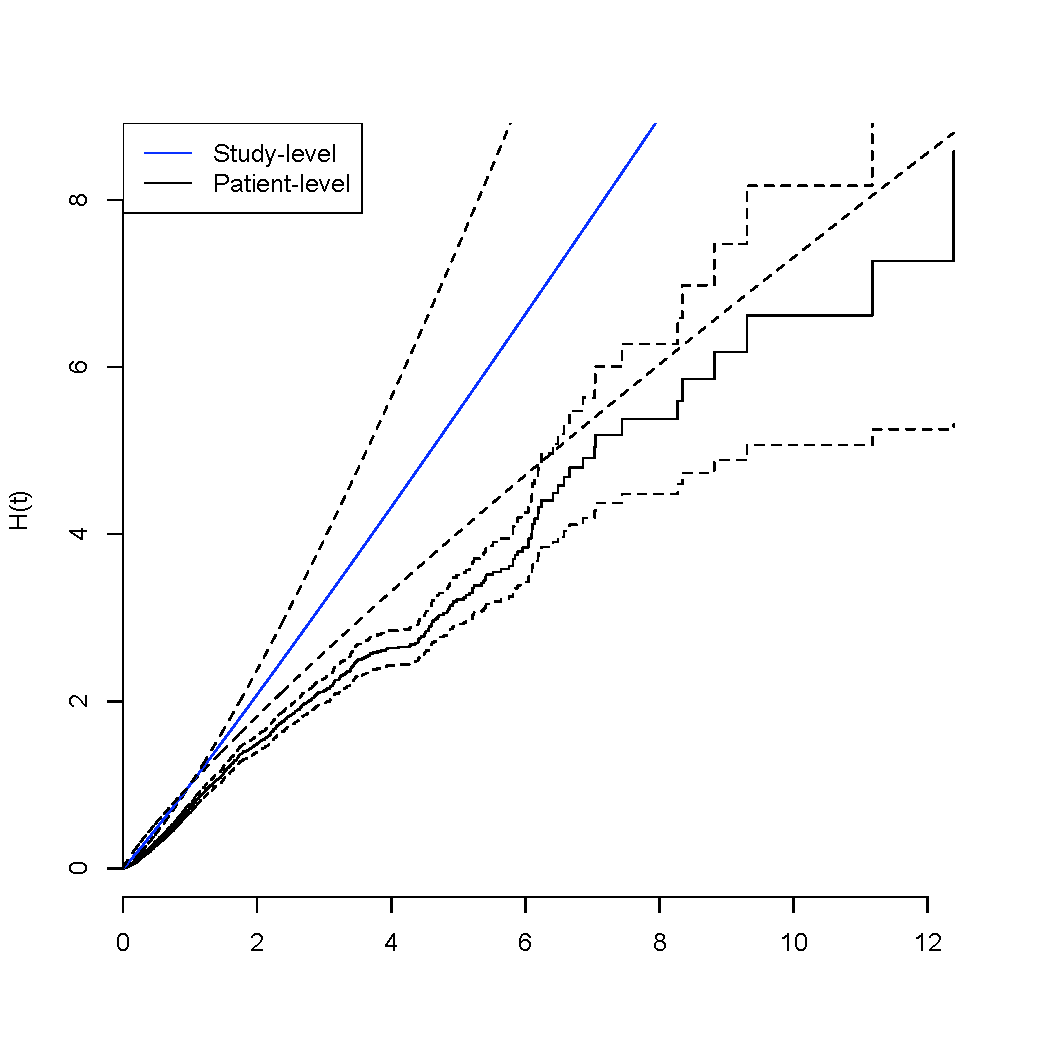
\includegraphics{haz.pdf}
\caption{Baseline hazard estimated by study-level and patient-level
  models of mixed-level meta-analysis. Dotted lines denote the 95\% CI.}
\end{figure}

\clearpage

\label{ref:ref}

\bibliographystyle{wileyj}

\bibliography{/Users/skoval/meta/bib/survival,/Users/skoval/meta/bib/survival.meta,/Users/skoval/meta/bib/statistics,/Users/skoval/meta/bib/meta,/Users/skoval/meta/bib/ecological_bias,/Users/skoval/meta/bib/likelihood,/Users/skoval/meta/bib/bayes.meta,/Users/skoval/meta/bib/bayes,/Users/skoval/meta/bib/power_loss,/Users/skoval/meta/bib/cox_randomeffects,/Users/skoval/meta/bib/importance_sampling,/Users/skoval/bibliography/public_health,/Users/skoval/bibliography/cer,/Users/skoval/meta/bib/bhits}


\end{document}
